\chapter{Results}
\label{chap:results}

\section{Deduplication}
It is clear that $\scheme$ enables deduplication since different users with the same file will end up with the same tag and therefore only one copy is saved in the server. We will now state two theorems regarding the privacy and security of $\scheme$ 

\section{Recovery}
\begin{theorem}
	If $\mathcal{E}$ is a correct deterministic symmetric encryption (D-SE) and $\mathsf{H}$ is collision resistant, then the above scheme $\scheme [\mathsf{H},\mathcal{E}, C]$ is \textsc{Rec}-secure.
\end{theorem}
\subsubsection*{Proof}
For adversary $A$ to win the \textsc{Rec} game, there must be a mismatch in the plaintext $m$ put on the server and the plaintext $m'$ recovered using $\mathsf{Get}$.\\ 
Whenever the client sends the ciphertext $C=(C_\psi, \Delta)$, the tag $t=(t_1, t_2)$ is computed by the server and \textbf{fil}[$t_1$], \textbf{delt}[$t_2$] and \textbf{own}[$t$] are filled. Since the tables are immutable, the ciphertext will not change once it is entered. When the client requests for tag $t$, the server checks \textbf{own}[$t$] and returns \textbf{fil}[$t_1$] and \textbf{delt}[$t_2$]. Thus recovery correctness is always ensured except when a collision occurs. Since we are using a collision resistant hash function, the probability of this happening is negligible.

\section{Privacy}
\begin{definition}
	The error-correcting code $C=(\msgspc, K, \tau)$ is said to be compatible with a source $\mathsf{S}$ with min-entropy $\mu(\secpar)$ iff $2^{\mu(\secpar)-\tau}$ is negligible.
	\label{def}
\end{definition}
This definition is used to put a constraint on the error correcting distance of $C$. If the error correcting distance $\tau$ is large, we cannot ensure privacy. This is because we are leaking $\Delta$ which has an entropy bounded by $\tau$. Thus even after leaking $\tau$ bits of information, there needs to be enough entropy in the message space to ensure unpredictability.

\begin{theorem}
	If $\mathcal{E}$ is CPA-secure and KR-secure and the code $C=(\msgspc, K, \tau)$ is compatible with the source $S$, then $\scheme_{RO}$[$\mathcal{E}$, $C$] \footnote{$\scheme_{RO}$ is the ROM analogue of $\scheme$ which models $\mathsf{H}$ as a random oracle} is \textsc{Priv}-secure.
\end{theorem}

\subsubsection*{Proof}
In the \textsc{Priv} game, the source $S$ outputs two vectors $\textbf{m}_0, \textbf{m}_1$ where $\textbf{m}_i$ is a vector over $\bin^*$. A random bit $b$ is chosen. Adversary can put and get components of $\textbf{m}_b$ and finally learns the server-side state. $A$ wins if it correctly guesses b.\\

Let $\mathsf{S}$ be an unpredictable PT source and $C$ be a compatible error correcting coding scheme. $\mathsf{S}$ outputs $m(\secpar)$ plaintexts each of length $\ell(\secpar, i)$. We denote the polynomial time adversary using $A$. The number of messages stored by the adversary is bounded by $n: \NN \rightarrow \NN$ and the number of random oracle queries made by source and adversary is bounded by $q_S(\secpar): \NN \rightarrow \NN $ and $q_A(\secpar): \NN \rightarrow \NN $
\\ 
We will use a hybrid argument to show the privacy of the $\scheme$. Consider the \textsc{Priv} game in the figure \ref{fig:priv}.\\
\begin{figure}
	\centering
	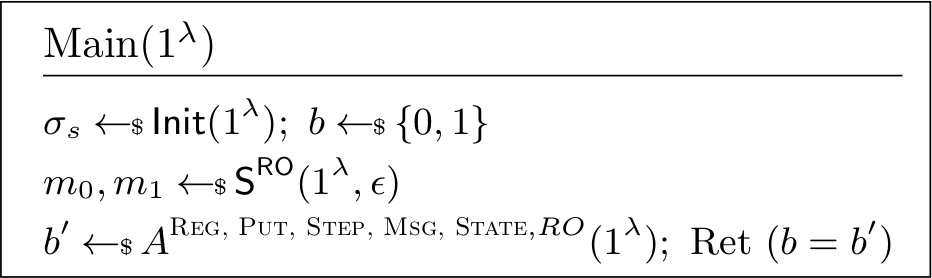
\includegraphics[scale=0.3]{Priv_game}
	\caption{The \textit{main} function of the \textsc{Priv} game}
	\label{fig:priv}
\end{figure}

\begin{figure}
	\centering
	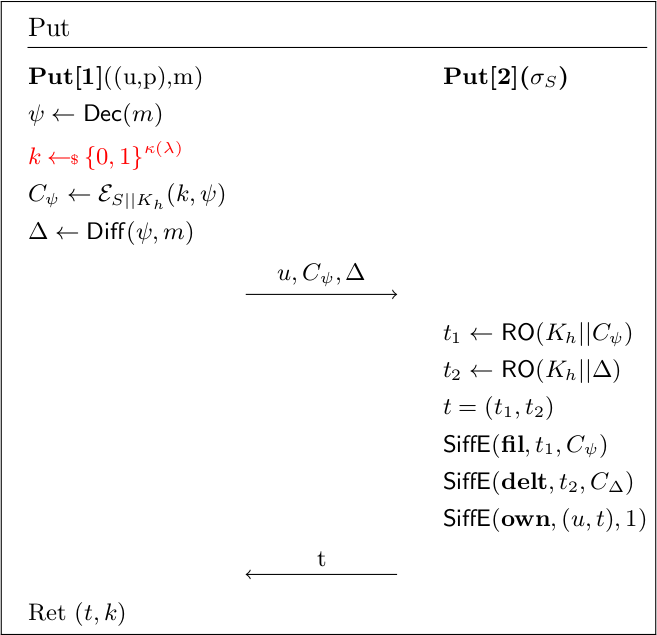
\includegraphics[scale=0.4]{H2}
	\caption{The $\mathsf{Put}$ protocol in game $H_2$}
\end{figure}

\begin{figure}
	\centering
	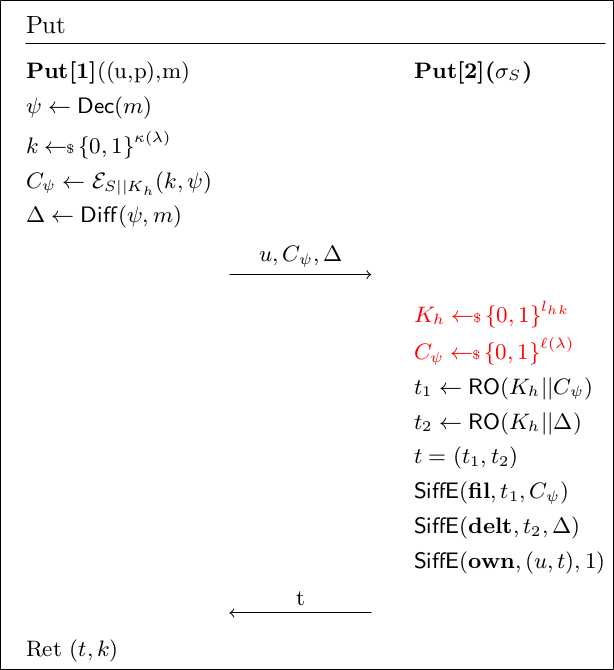
\includegraphics[scale=0.4]{H3}
	\caption{The $\mathsf{Put}$ protocol in game $H_3$}
\end{figure}

\noindent
The \textsc{Reg, Step, Msg} and \textsc{State} are same as in the \textsc{Priv} game. The $\mathsf{Put}$ protocol changes in each hybrid game.
Let $H_1$ denote the actual $\mathsf{Put}$ protocol from figure \ref{fig:put} with the only difference being that instead of $H$, it uses $RO$. In the game $H_2$, the $k$ is sampled randomly instead of using the extractor output. This will give the adversary with an $\epsilon$ advantage since the extractor output is $\epsilon$ close to uniform distribution.

\begin{equation}
\prob{\textsc{Priv}_\scheme^{\mathsf{S,A}}(a^\lambda)} = \prob{H_1^{\mathsf{S,A}}} \leq \prob{H_2^{\mathsf{S,A}}} + \epsilon
\end{equation}

In $H_3$, the RO queries for $t_1$ are made using random strings. The adversary can detect this only if it had queried $\mathsf{RO}(K_h||C_\psi)$. The probability for this bad event is bounded by $q_A(\lambda)n(\lambda)/2^{\ell(\secpar, i) - \tau}$ where $q_A$ is the bound on the number of RO queries made by $A$.

\begin{equation}
\prob{H_2^{S,A} \text{ sets }\mathsf{bad}} -
\prob{H_3^{S,A} \text{ sets }\mathsf{bad}}  \leq \frac{q_A(\lambda)n(\lambda)}{2^{m(\secpar) - \tau}}  + q_s(\lambda)n(\lambda)GP_S(\lambda)
\end{equation}

In game $H_4$, $\psi$ is an encryption of a random string. The CPA-security of the $\mathit{Enc}$ means that adversary cannot distinguish with any significant advantage. In game $H_4$, there is no information about the message $m$ at all other than $\Delta$. By Definition \ref{def}, the min-entropy of the message $m$ is still high. Thus,

\begin{equation}
\prob{H_4^{A} \text{ sets }\mathsf{bad}} \leq  \frac{q_A(\lambda)n(\lambda)}{2^{m(\secpar) - \tau}} + q_s(\lambda)n(\lambda)GP_S(\lambda)
\end{equation}

\begin{figure}[H]
	\centering
	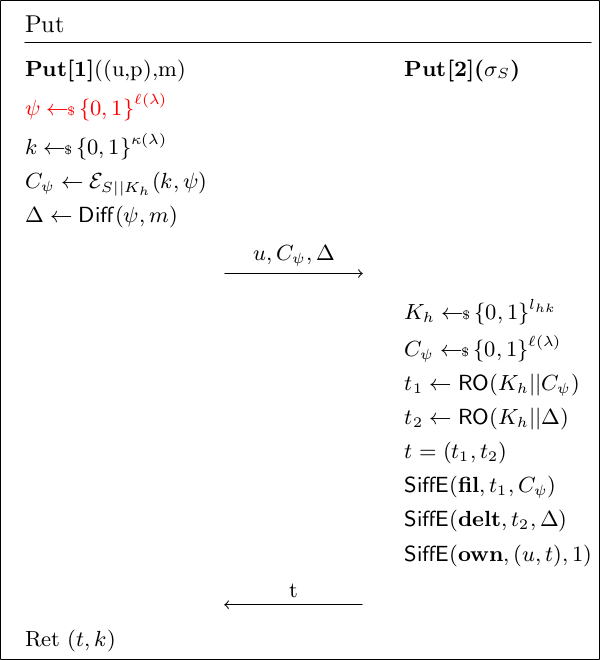
\includegraphics[scale=0.5]{H4}
	\caption{The $\mathsf{Put}$ protocol in game $H_4$}
\end{figure}        

Since at each of the hybrid steps there is only a negligible hit in the probability of adversary winning, adding all the probabilities will still give only a negligible advantage to the adversary. Thus $\scheme$ is \textsc{Priv}-secure.\\ \\
The scheme is efficient since when files that are close together are uploaded, the storage grows only by an additional factor of $\Delta$ for each new file. If the files are identical, then the overhead is minimal.